% IEEE standard conference template; to be used with:
%   spconf.sty  - LaTeX style file, and
%   IEEEbib.bst - IEEE bibliography style file.
% --------------------------------------------------------------------------

\documentclass[letterpaper]{article}
\usepackage{spconf,amsmath,amssymb,graphicx}
\usepackage{graphicx}
\usepackage{tabularx}
\usepackage[export]{adjustbox}
\usepackage{float}
\usepackage{array}


% Example definitions.
% --------------------
% nice symbols for real and complex numbers
\newcommand{\R}[0]{\mathbb{R}}
\newcommand{\C}[0]{\mathbb{C}}

% bold paragraph titles
\newcommand{\mypar}[1]{{\bf #1.}}

% Title.
% ------
\title{Predictions of urban qualities in the city of Zurich}
%
% Single address.
% ---------------
\name{Jakub Lichman, Philippe Schlattner, Florian Koch}
\address{Department of Computer Science\\ ETH Zurich\\Zurich, Switzerland}

% For example:
% ------------
%\address{School\\
%		 Department\\
%		 Address}
%
% Two addresses (uncomment and modify for two-address case).
% ----------------------------------------------------------
%\twoauthors
%  {A. Author-one, B. Author-two\sthanks{Thanks to XYZ agency for funding.}}
%		 {School A-B\\
%		 Department A-B\\
%		 Address A-B}
%  {C. Author-three, D. Author-four\sthanks{The fourth author performed the work
%		 while at ...}}
%		 {School C-D\\
%		 Department C-D\\
%		 Address C-D}
%

\begin{document}
%\ninept
%
\maketitle
%

\begin{abstract}


\end{abstract}

\section{Introduction}\label{sec:intro}
Huge increase in number of world urban area residents from 54 to 66 percent in 2050 brings many challenges which every successful city has to overcome. 
There are many factors that influence one's impression of the city. Most notable are availability of public transport, pollution, streets illumination, greenery, pedestrian zones, cycling routes etc. However quality of these factors usually varies within a city. Different districts provide different pros and
cons and thus deciding on which part of the city is best for an individual is not trivial.

\section{Background}\label{sec:background}

 \begin{figure}
	\centering
	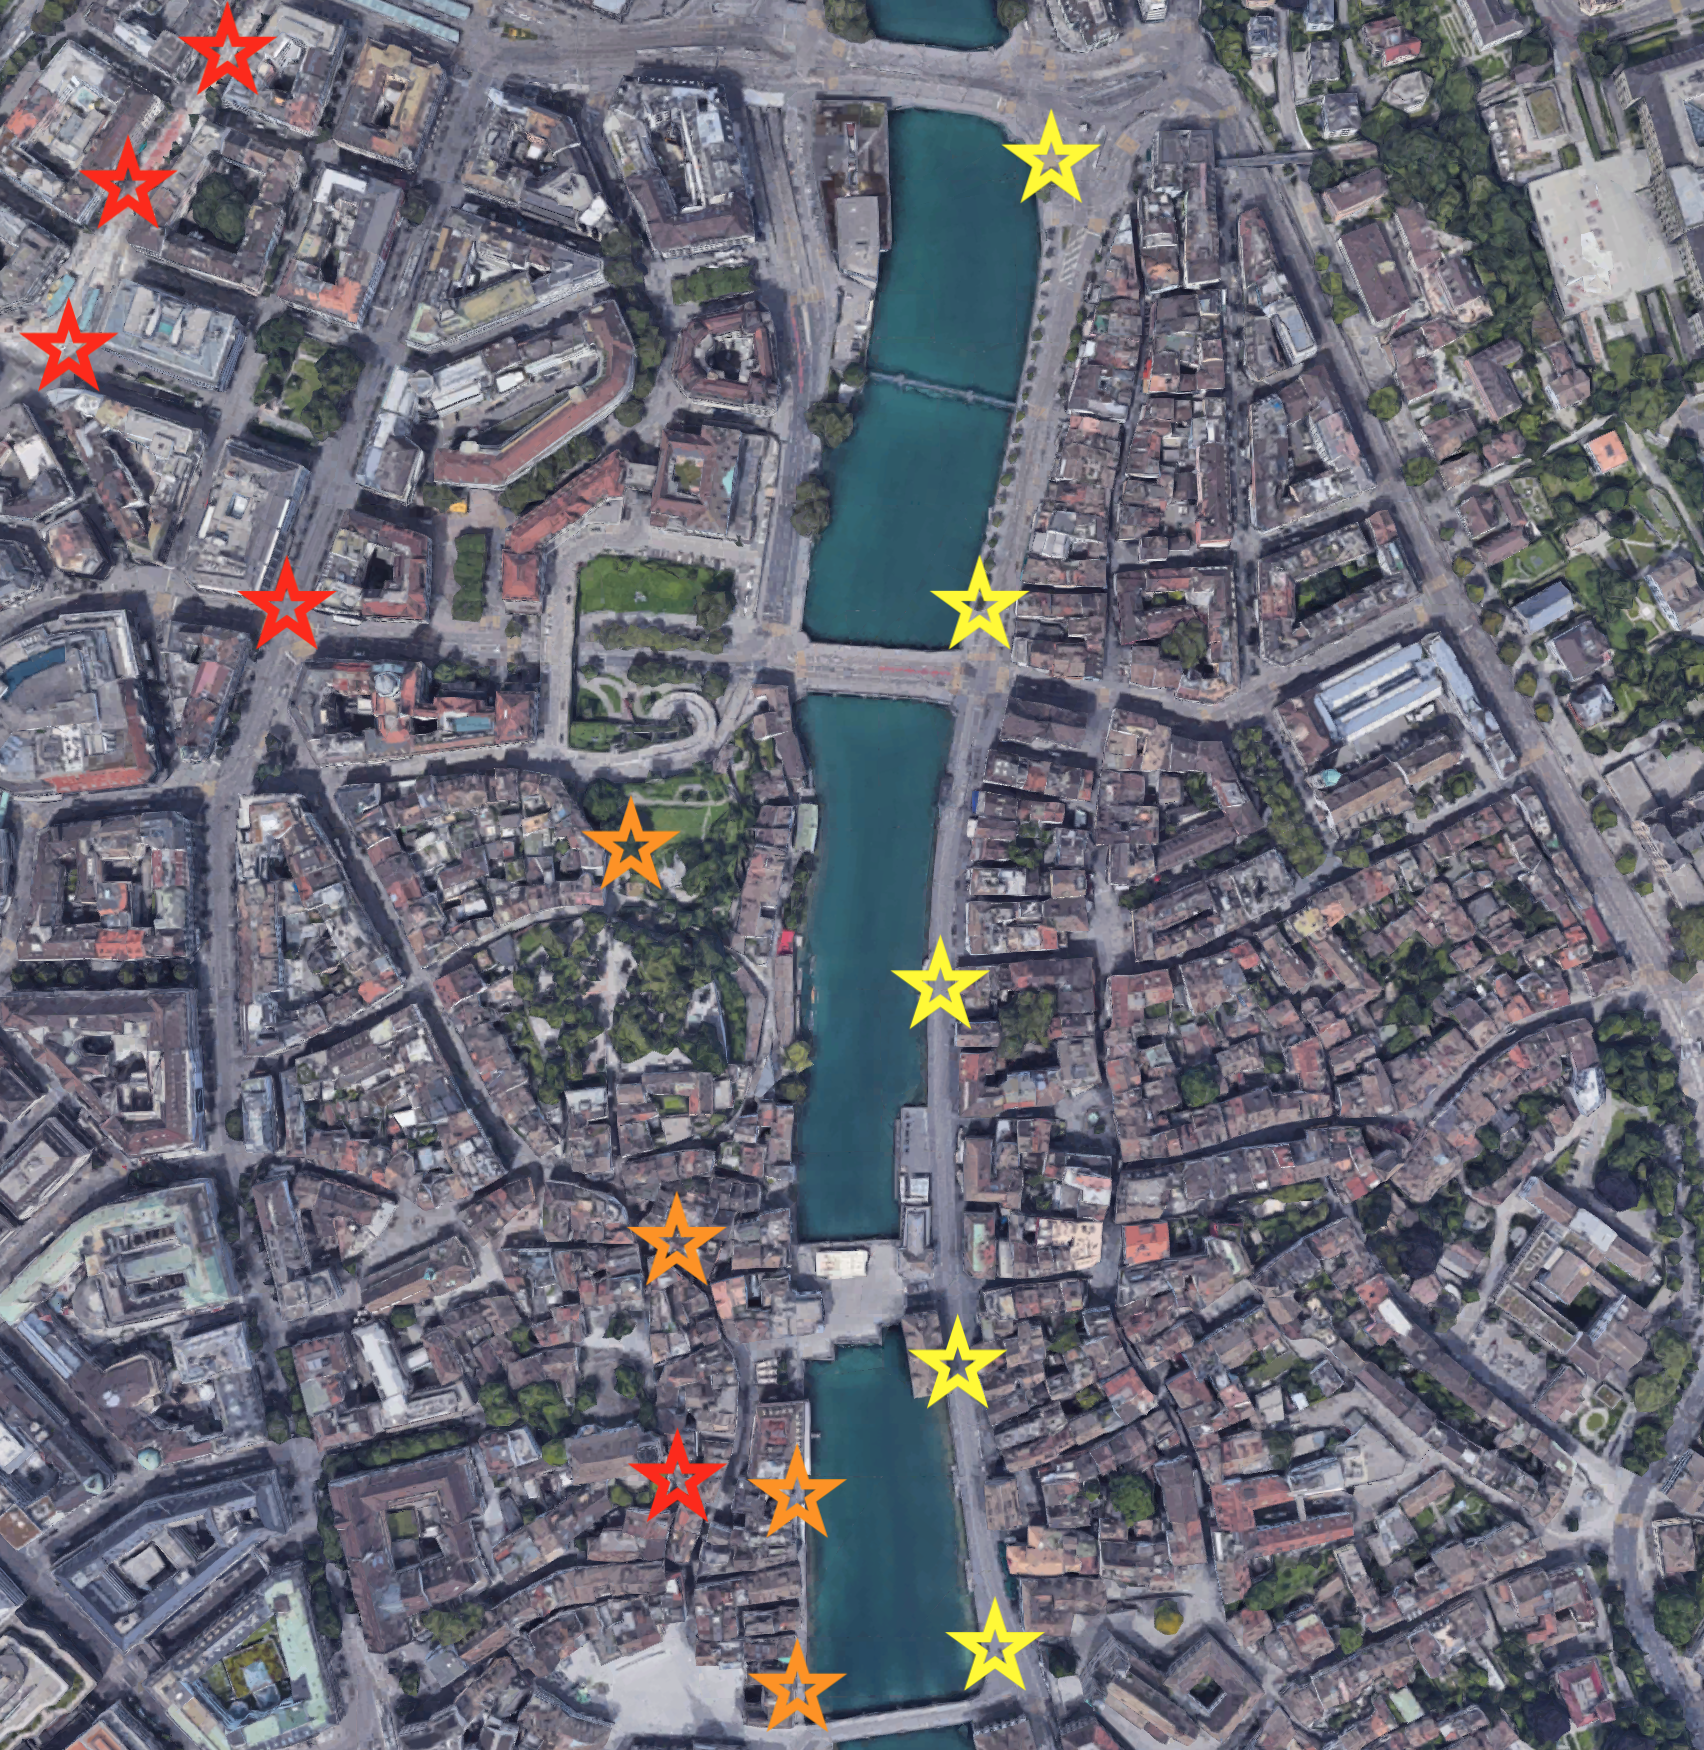
\includegraphics[width=\columnwidth]{../images/greenery/Zentrum_path.png}
	\caption{Locations of question points along the path}
	\label{fig:path_points}
\end{figure}

\section{Greenery Detection}\label{sec:greenery}

\indent Greenery has always played crucial part in the construction of cities. The need for green spaces has been present since ancient times. 
City parks are traditional place of recreation and relax for all kinds of people in their spare time. Current trends in architecture brought new ways of
connection between buildings and greenery such as roofs with green surfaces or terraces with tree pots. These trends are consequence of natural human inclination towards nature. Therefore we have decided to take greenery as a significant indicator of urban quality. 

\indent In order to predict user preferences partially based on greenery, we needed to acquire data about it. There are two basic ways how to detect trees, parks or grass areas on a map. First approach relies on a snapshot of a satellite view \cite{smartCities}. It is simple to implement and yield accurate results. Detection of green areas is via pixels with RGB values that lie within specified intervals. The only crucial requirement in order to obtain precise detection is to find high quality satellite view of the selected area.
Second approach is to detect greenery from Google Street View (GSV) \cite{googleView}. Xiaojiang Li et. al. detected greenery by examining street
pictures taken from GSV. With this method they were able to explore greenery inside the cities in great detail. Idea behind second method is in general
more accurate since it can detect trees shadowed by taller buildings or shelters. However, its precision highly depends on availability of street view and
algorithms, which are in our view still not accurate enough. That is the reason why we have decided to use the first method.
 
  \begin{figure}
 	\centering
 	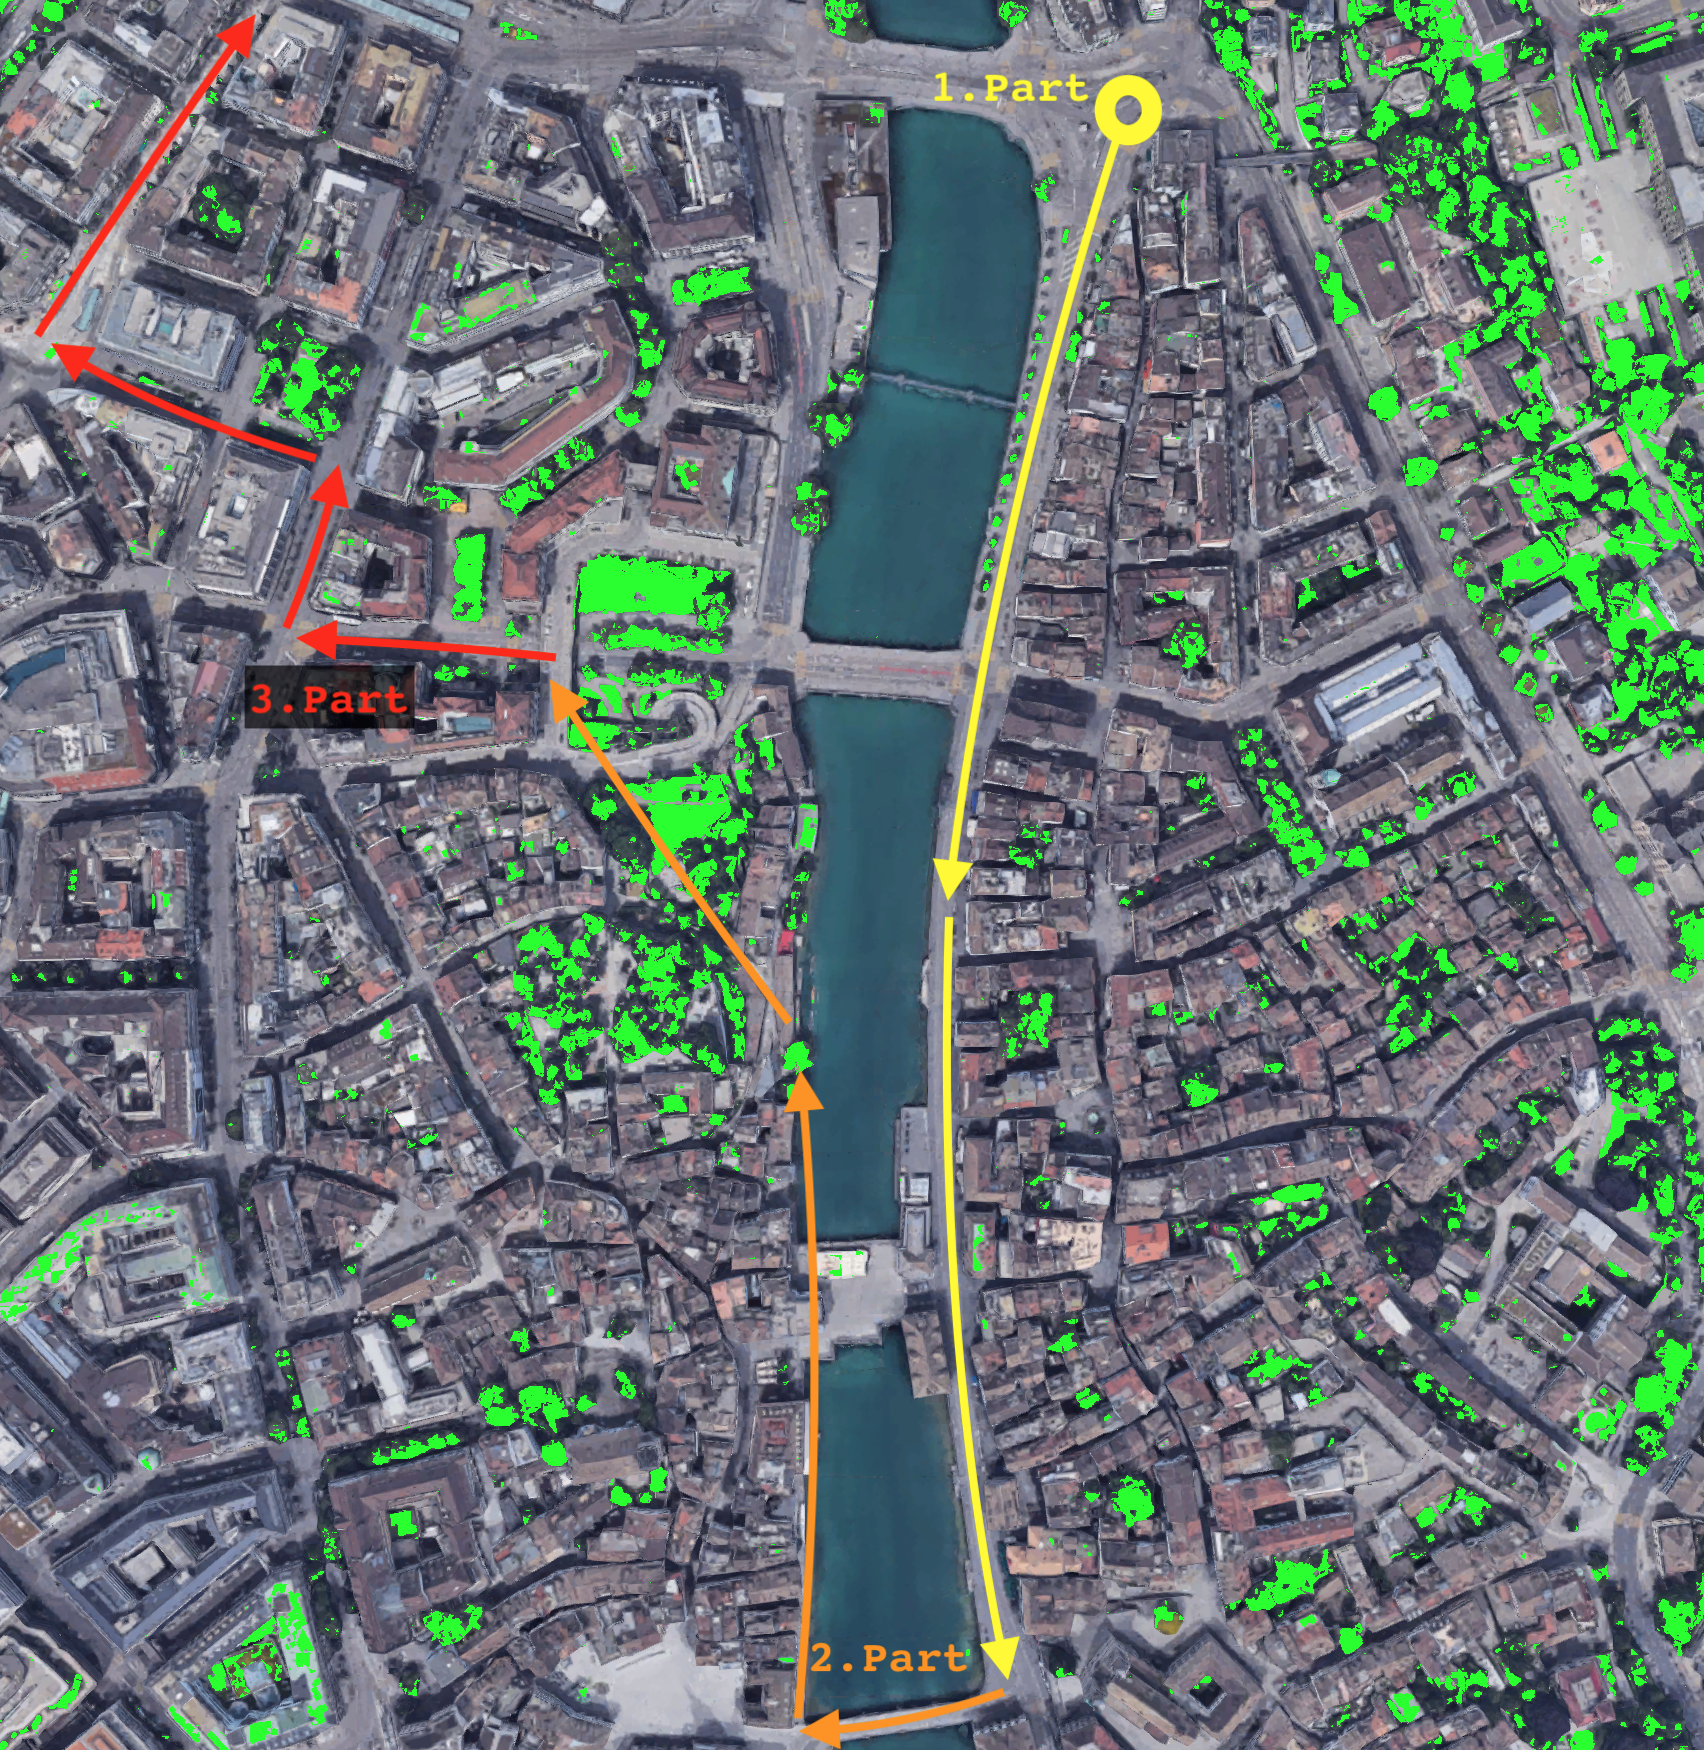
\includegraphics[width=\columnwidth]{../images/greenery/Zentrum_greenery.png}
 	\caption{Greenery detection in the area of our path.}
 	\label{fig:path_greenery}
 \end{figure}

\indent We have developed python script which does greenery detection similarly to the first approach mentioned above. It detects green pixels and marks them with RGB value (0, 255, 0). Snapshot of selected location was taken from Google maps satellite view which satisfies our quality requirements.  %Such a method is capable of detecting 
 

\section{Experimental Results}\label{sec:exp}

\section{Discussion}\label{sec:discussion}


\section{Conclusion}\label{sec:conclusion}

\bibliographystyle{IEEEbib}
\bibliography{bibl_conf}

\newpage
\section{Appendix}

\end{document}
